%%%%%%%%%%%%%%%%%%%%%%%%%%%%%%%%%%%%%%%%%
% Short Sectioned Assignment LaTeX Template Version 1.0 (5/5/12)
% This template has been downloaded from: http://www.LaTeXTemplates.com
% Original author:  Frits Wenneker (http://www.howtotex.com)
% License: CC BY-NC-SA 3.0 (http://creativecommons.org/licenses/by-nc-sa/3.0/)
%%%%%%%%%%%%%%%%%%%%%%%%%%%%%%%%%%%%%%%%%

%----------------------------------------------------------------------------------------
%   PACKAGES AND OTHER DOCUMENT CONFIGURATIONS
%----------------------------------------------------------------------------------------

\documentclass[10pt,a4paper,spanish]{article}

% ---- Entrada y salida de texto -----

\usepackage[spanish]{babel} 
\usepackage[T1]{fontenc} % Use 8-bit encoding that has 256 glyphs
\usepackage[utf8]{inputenc}
\usepackage{minted}
% \usepackage{fourier} % Use the Adobe Utopia font for the document - comment this line to return to the LaTeX default
\usepackage[usenames, dvipsnames]{color}
\usepackage{xcolor}
\usepackage{colortbl}
\usepackage[bookmarks=true,colorlinks=true,linkcolor=red,citecolor=blue]{hyperref}
\usepackage{cite}
\usepackage[official]{eurosym}
\usepackage{tikz}
\usepackage{pgfplots}
\pgfplotsset{compat=1.5}
% \usepackage{pgf-pie}
\usepackage{subfigure}

% ---- Otros paquetes ----
\usepackage{enumerate}
\usepackage{amsmath,amsfonts,amsthm,amssymb} % Math packages
\usepackage{graphics,graphicx} %para incluir imágenes y notas en las imágenes
% Para hacer tablas comlejas
%\usepackage{multirow}
%\usepackage{threeparttable}

\usepackage[a4paper, margin=1.3in]{geometry}


\usepackage{sectsty} % Allows customizing section commands
\allsectionsfont{\centering \normalfont\bfseries\scshape} % Make all sections centered, the default font and small caps

\usepackage{fancyhdr} % Custom headers and footers
\pagestyle{fancyplain} % Makes all pages in the document conform to the custom headers and footers
\fancyhead{} % No page header - if you want one, create it in the same way as the footers below
\fancyfoot[L]{} % Empty left footer
\fancyfoot[C]{} % Empty center footer
\fancyfoot[R]{\thepage} % Page numbering for right footer
\renewcommand{\headrulewidth}{0pt} % Remove header underlines
\renewcommand{\footrulewidth}{0pt} % Remove footer underlines
\setlength{\headheight}{13.6pt} % Customize the height of the header

\numberwithin{equation}{section} % Number equations within sections (i.e. 1.1, 1.2, 2.1, 2.2 instead of 1, 2, 3, 4)
\numberwithin{figure}{section} % Number figures within sections (i.e. 1.1, 1.2, 2.1, 2.2 instead of 1, 2, 3, 4)
\numberwithin{table}{section} % Number tables within sections (i.e. 1.1, 1.2, 2.1, 2.2 instead of 1, 2, 3, 4)

\setlength\parindent{0pt} % Removes all indentation from paragraphs - comment this line for an assignment with lots of text
\setlength{\parskip}{1ex plus 0.5ex minus 0.2ex}

\newcommand{\horrule}[1]{\rule{\linewidth}{#1}} % Create horizontal rule command with 1 argument of height

%----------------------------------------------------------------------------------------
%   TÍTULO Y DATOS DEL ALUMNO
%----------------------------------------------------------------------------------------

\title{
\normalfont \normalsize 
\textsc{{\bf Ingeniería de Servidores (2015-2016)} \\ Grado en Ingeniería Informática \\ Universidad de Granada} \\ [25pt] % Your university, school and/or department name(s)
\horrule{0.5pt} \\[0.4cm] % Thin top horizontal rule
\huge Cuestiones Opcionales \\ % The assignment title
\horrule{2pt} \\[0.5cm] % Thick bottom horizontal rule
}

\author{Marta Gómez Macías} % Nombre y apellidos

\date{\normalsize\today} % Incluye la fecha actual

\newmintedfile[mypython]{python}{
    linenos,
    numbersep=5pt,
    gobble=0,
    frame=lines,
    framesep=2mm,
    tabsize=3,
}

%----------------------------------------------------------------------------------------
% DOCUMENTO
%----------------------------------------------------------------------------------------

\begin{document}
%Cambiar Cuadros por Tablas y lista de...
\renewcommand{\listtablename}{Índice de tablas}
\renewcommand{\tablename}{Tabla} 

\maketitle % Muestra el Título
\pagenumbering{gobble} 

\newpage %inserta un salto de página
\pagenumbering{arabic} 

\tableofcontents % para generar el índice de contenidos

\listoffigures

% \listoftables

\newpage

\section{Práctica 1}
\subsection{Muestre (con capturas de pantalla) cómo ha comprobado que el RAID1 funciona.}
Tras eliminar el disco 1 de la máquina virtual e iniciar el sistema, comprobamos que al arrancar obtenemos la pantalla de la \hyperref[raid1]{Figura \ref*{raid1}}

\begin{figure}[!h]
\centering
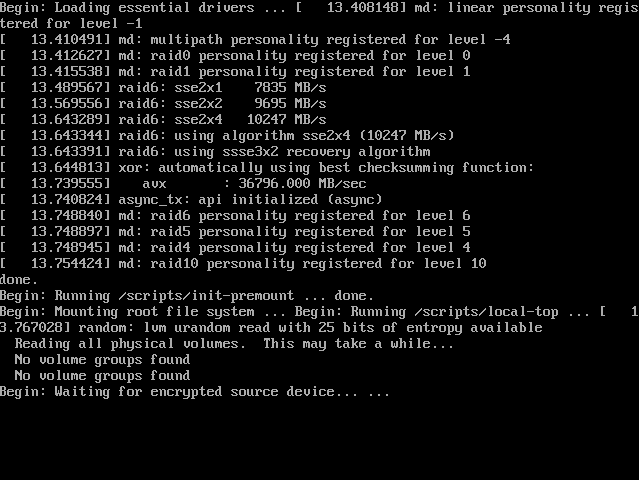
\includegraphics[width=0.8\textwidth]{1_7}
\caption{Pantalla al arrancar por primera vez habiendo quitado el disco 1}
\label{raid1}
\end{figure}

Tras esto, se iniciará el modo \texttt{initramfs}, en el que podremos ejecutar las instrucciones que se ven en la \hyperref[initramfs]{Figura \ref*{initramfs}} (obtenidas al pulsar el tabulador)

\begin{figure}[!h]
\centering
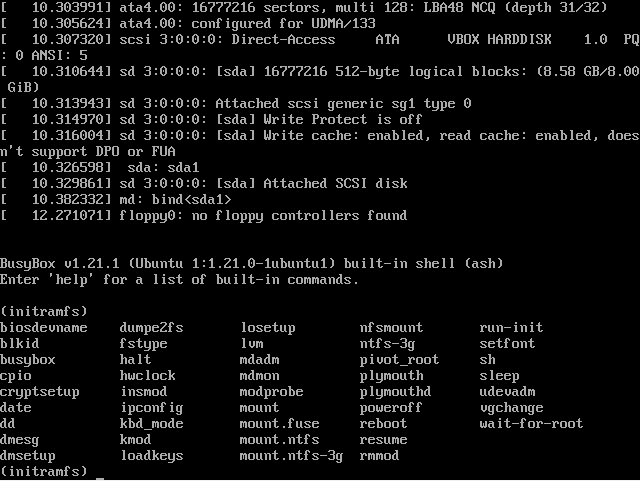
\includegraphics[width=0.8\textwidth]{1_8}
\caption{Pantalla al iniciarse \texttt{initramfs} y pulsar tabulador}
\label{initramfs}
\end{figure}

Comprobamos, en primer lugar, el estado actual en el que se encuentra el RAID consultado el archivo \texttt{mdstat}. Como se ve en la \hyperref[inactive]{Figura \ref*{inactive}}, vemos que está desactivado.

\begin{figure}[!h]
\centering
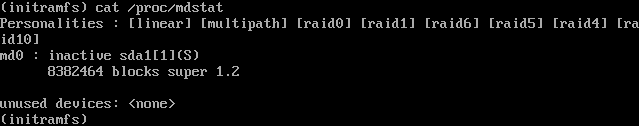
\includegraphics[width=0.8\textwidth]{1_10}
\caption{Comprobación del estado del RAID}
\label{inactive}
\end{figure}

Para activarlo, vamos a ejecutar \texttt{mdadm}, para ello ejecutamos tal y como se indica en las páginas man de \texttt{mdadm} (\cite{mdadm}):

\begin{minted}{bash}
mdadm -R /dev/md0
\end{minted}

Lo ejecutamos sobre md0, ya que estamos trabajando sobre el dispositivo RAID. Así, tal y como se ve en la \hyperref[active]{Figura \ref*{active}}, ya tenemos nuestro dispositivo RAID activado. 

Para terminar, pulsamos \textbf{Control+D} para seguir arrancando el sistema.

\begin{figure}[!h]
\centering
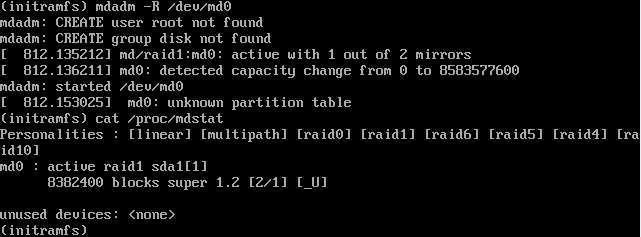
\includegraphics[width=0.8\textwidth]{1_9}
\caption{Activación del RAID y su posterior comprobación}
\label{active}
\end{figure}

\subsection{¿Qué relación hay entre los atajos de teclado de emacs y los de la consola de bash? ¿y entre los de vi y las páginas del manual?}
Tal y como se dice en \cite{keysemacs}, los atajos de teclado tanto en bash como en emacs son los mismos. También en \cite{keysemacs} nos ponen unos ejemplos de atajos de teclado de emacs para la consola de bash:
\begin{enumerate}[$\heartsuit$]
    \item \texttt{CTRL-P}: ir al comando anteriormente ejecutado en el historial
    \item \texttt{CTRL-N}: ir al siguiente comando ejecutado en el historial
    \item \texttt{CTRL-R}: buscar en el historial de comandos ejecutados al revés
    \item \texttt{CTRL-S}: según la página es buscar en el historial de comandos, pero a mí me suspende la terminal y tengo que pulsar \texttt{CTRL-Q} para volverla a iniciar.
    \item \texttt{CTRL-A}: mover el cursor al inicio de la línea.
    \item \texttt{CTRL-E}: mover el cursor al final de la línea
    \item \texttt{CTRL-W}: eliminar la última palabra en la que se encuentra el cursor. Por ejemplo, en el comando \texttt{bibtex citas}, eliminaría la palabra \texttt{citas}.
    \item \texttt{ALT-D}: eliminar la siguiente palabra a la que apunta el cursor. Por ejemplo, si tenemos el cursor al inicio de la línea, se eliminaría la primera palabra.
    \item \texttt{CTRL-F}: mover el cursor un carácter hacia delante.
    \item \texttt{CTRL-B}: mover el cursor un carácter hacia atrás.
    \item \texttt{ALT-F}: mover el cursor una palabra hacia delante.
    \item \texttt{ALT-B}: mover el cursor una palabra hacia detrás.
    \item \texttt{ALT-\_}: escribir la última palabra que has escrito en el historial.
\end{enumerate}

Lo mismo pasa con \texttt{vi} y las \texttt{man pages}. Por ejemplo, en la \hyperref[man]{Figura \ref*{man}} vemos los comandos para movernos por una página de manual, pero, esos mismos comandos también nos sirven para movernos por un archivo abierto con vi, pero combiándolos con la tecla control.

\begin{figure}[!h]
\centering
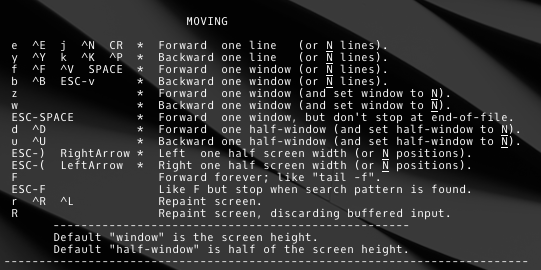
\includegraphics[width=0.5\textwidth]{1_20}
\caption{Comandos para moverse a través de una página de manual}
\label{man}
\end{figure}

\section{Práctica 2}
\subsection{¿Qué gestores utiliza OpenSuse?}
En la sección \textit{Gestor de paquetes} de \cite{wikisuse} se explica que hay dos gestores de paquetes en openSUSE:
\begin{enumerate}[$\bullet$]
    \item \textbf{YaST}: es un gestor de paquetes con interfaz gráfica.
    \item \textbf{Zypper}: es un gestor de paquetes desde la línea de comandos. En \cite{zypper} podemos encontrar una guía de uso de este gestor de paquetes.
\end{enumerate}

\subsection{Instale y pruebe terminator. Con screen, pruebe su funcionamiento dejando sesiones ssh abiertas en el servidor y recuperándolas posteriormente}
Mi experiencia con terminator se resume en la \hyperref[terminator]{Figura \ref*{terminator}}. He probado a partir la pantalla, poner un perfil distinto en cada división y, trabajar en tareas independientes en cada terminal de forma paralela.

\begin{figure}[!h]
\centering
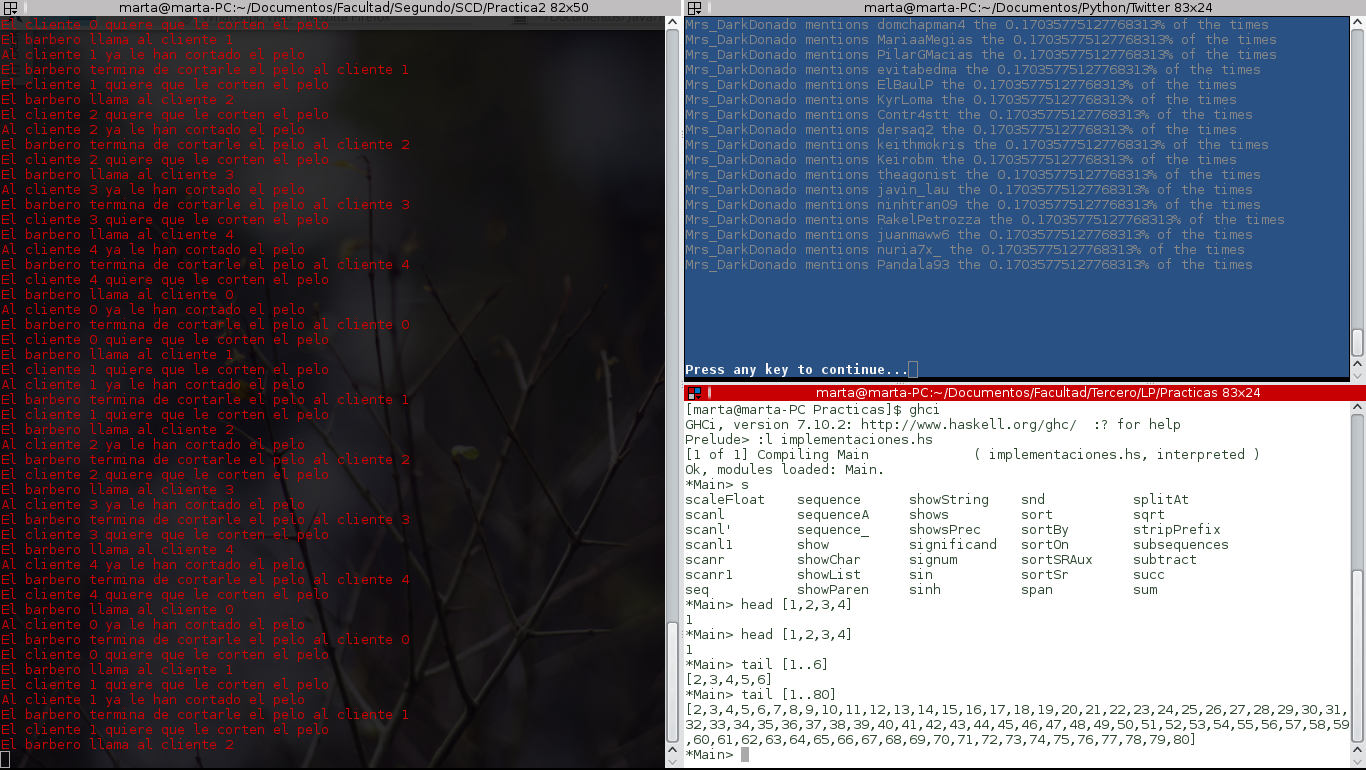
\includegraphics[width=0.75\textwidth]{2_16}
\caption{Prueba con terminator}
\label{terminator}
\end{figure}

En \cite{screen}, se explica un funcionamiento básico de screen. En nuestro caso, tendremos dos sesiones de screen abiertas.

Probamos a abrir una sesión ssh en la sesión 1, y pulsando \textbf{Control+a+d} la suspendemos. Tras esto, se cierra la sesión, pero podemos listar las sesiones de screen actualmente en funcionamiento con el comando:

\begin{minted}[frame=single, label={listando las sesiones de screen actuales}]{bash}
screen -ls
\end{minted}

\begin{figure}[!h]
\centering
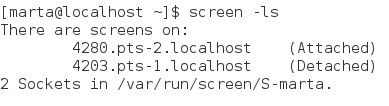
\includegraphics[width=0.75\textwidth]{2_51}
\caption{Listando las sesiones de \texttt{screen} actualmente abiertas}
\label{screenlist}
\end{figure}

Como se ve en la \hyperref[screenlist]{Figura \ref*{screenlist}} tenemos una sesión suspendida. Para recuperarla usamos la opción \texttt{-r} acompañada del ID de dicha sesión:

\begin{minted}[frame=single, label={Reanudando la sesión ssh que teníamos en screen}]{bash}
screen -r 4203 
\end{minted}

También probamos el modo de \textit{split window}. Para ello, pulsamos \textbf{Control+a+S}, tras esto, nos movemos a la nueva ventana que hemos hecho con \textbf{Control+a+Tab} y una vez ahí pulsamos \textbf{Control+a+c} para empezar una nueva sesión de screen. El resultado es el que se ve en la \hyperref[split]{Figura \ref*{split}}. 

\begin{figure}[!h]
\centering
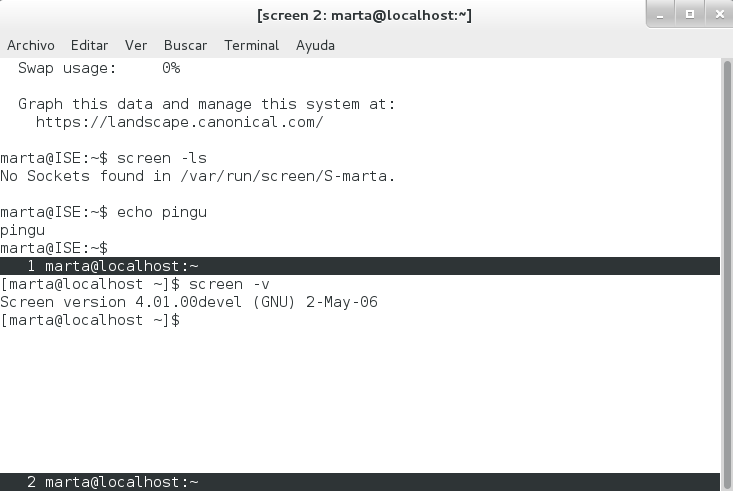
\includegraphics[width=0.75\textwidth]{2_17}
\caption{Haciendo un split en la sesión de screen actual}
\label{split}
\end{figure}

\subsection{Instale el servicio \texttt{fail2ban} y pruebe su funcionamiento}
Para instalar \texttt{fail2ban} en Ubuntu Server ejecutamos el comando bien conocido:
\begin{minted}[frame=single, label={Instalación de fail2ban en Ubuntu Server}]{bash}
sudo apt-get install fail2ban    
\end{minted}

Una vez hecho esto, consultamos \cite{fail2banwiki} para saber cómo se usa y cómo se configura. En primer lugar tenemos un cliente y un servidor:
\begin{enumerate}[---]
    \item \texttt{fail2ban-client}: es el \textit{frontend} de Fail2ban. Se conecta al servidor definido en el archivo socket y le envía comandos para configurar y operar el servidor. El cliente puede leer archivos de configuración o usarse para mandar órdenes al servidor. Sus opciones son:
    \begin{enumerate}[$\bullet$]
        \item \texttt{-c <DIR>}: directorio de configuración. Por defecto \textit{/etc/fail2ban}
        \item \texttt{-s <FILE>}: ruta del socket
        \item \texttt{-d}: configuración ``\textit{dump}'', para depurar.
        \item \texttt{-i}: modo interactivo
        \item \texttt{-v}: aumenta la cantidad de información que nos muestra el programa
        \item \texttt{-q}: disminuye la cantidad de información que nos muestra el programa
        \item \texttt{-x}: fuerza la ejecución del servidor
        \item \texttt{-h}: ayuda
        \item \texttt{-V}: muestra la versión
    \end{enumerate}
    \item \texttt{fail2ban-server}: el servidor inicialmente no tiene definida ninguna ``cárcel''. No debe usarse directamente, excepto cuando se está depurando. Dispone de las siguientes opciones:
    \begin{enumerate}[$\bullet$]
        \item \texttt{-b}: empieza el programa en segundo plano
        \item \texttt{-f}: empieza el programa en primer plano
        \item \texttt{-s <FILE>}: ruta del socket
        \item \texttt{-x}: fuerza la ejecución del servidor
        \item \texttt{-h}: muestra un mensaje de ayuda
        \item \texttt{-V}: muestra la versión
    \end{enumerate}
\end{enumerate}

Para hacer una simple prueba, iniciamos \texttt{fail2ban} con la configuración por defecto:
\begin{minted}[frame=single, label={Iniciamos fail2ban}]{bash}
sudo fail2ban-client -v start
\end{minted}

Como información nos da que el archivo socket en uso es \textit{/var/run/fail2ban/fail2ban.sock}.

Si usamos la opción \texttt{-i}, nos saldrá algo parecido a cuando usamos ftp para introducir comandos, \texttt{fail2ban>}.

Si miramos el archivo \textit{jail.conf}, podemos configurar cosas tales como las IP que no queremos banear, el tiempo que un host queda baneado, los parámetros para banear a un host (número de peticiones que genera en un tiempo determinado), etc. 

También podemos configurar los distintos servicios que queremos controlar, por ejemplo: ssh, xinetd, apache, vsftp, etc.

% \subsection{Realice la instalación de uno de estos dos ``web containers'' (\textit{Apache Tomcat} o \textit{Jboss}) y pruebe su ejecución.}

% Hemos elegido el \textit{Apache Tomcat}. Para descargarlo hemos entrado en \href{http://tomcat.apache.org/download-80.cgi}{Download Tomcat 8.0}, en el menú de la izquierda. Una vez ahí, hemos escogido la versión para Windows de 64 bits.

% Una vez descargado, abrimos el archivo \textbf{RUNNING}, en el cual se nos indica que para ejecutar el programa debemos tener instalado \href{http://www.oracle.com/technetwork/java/javase/downloads/index.html}{Java SE Runtime Environment (JRE)}.

\setcounter{subsection}{5}

% \subsection{Realice la instalación de MongoDB en alguna de sus máquinas virtuales. Cree una colección de documentos y haga una consulta sobre ellos.}
% Siguiendo los pasos indicados en \cite{installmongo}:
% \begin{enumerate}[1.]
% \item En primer lugar creamos el archivo de repositorio de MongoDB para ello ejecutamos el siguiente comando:
% \begin{minted}[frame=single, label={Creando el archivo de repositorio de MongoDB}]{bash}
% sudo touch /etc/yum.repos.d/mongodb-org-3.0.repo
% \end{minted}

% \item Le damos contenido al archivo, en concreto el contenido que se ve en la \hyperref[repo]{Figura \ref*{repo}}.

% \begin{minted}[frame=single, label={Dando contenido al archivo}]{bash}
% sudo nano /etc/yum.repos.d/mongodb-org-3.0.repo
% \end{minted}

% \begin{figure}[!h]
%     \centering
%     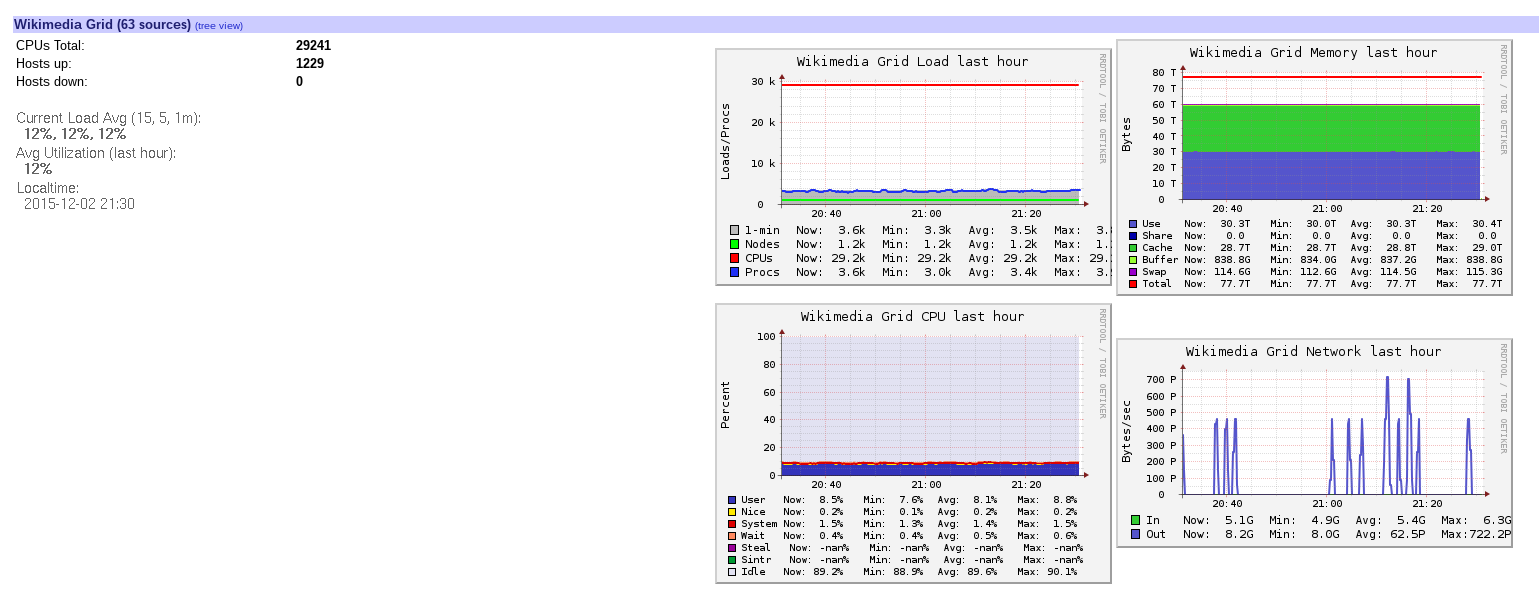
\includegraphics[width=0.7\textwidth]{50}
%     \caption{Contenido del archivo de configuración del repositorio de MongoDB}
%     \label{repo}
% \end{figure}

% \item Tras esto, instalamos MongoDB con \texttt{yum}:
% \begin{minted}[frame=single, label={Instalando MongoDB}]{bash}
% sudo yum install -y mongodb-org
% \end{minted}

% \item Una vez instalado, debemos configurar SELinux para permitir que MongoDB arranque. Para ello, establecemos el parámetro \texttt{SELINUX} del archivo \textit{/etc/selinux/config} a \texttt{permissive}.
% \begin{minted}[frame=single, label={Configurando SELinux}]{bash}
% sudo nano /etc/selinux/config
% SELINUX=permissive
% \end{minted}

% \item Reiniciamos el sistema.

% \item Iniciamos el servicio, para ello usamos el siguiente comando:
% \end{enumerate}

\subsection{Muestre un ejemplo de uso para \texttt{awk}}
En \cite{manawk} se ponen algunos ejemplos de uso de \texttt{awk}. Un ejemplo es \textit{preceder cada línea de su número en un archivo}. Esto se haría con el siguiente comando \texttt{awk}:
\begin{minted}[frame=single, label={Añadiendo a cada linea su numero de linea}]{bash}
awk -F: '{ nlines++; print nlines, $0; }' hola.txt
\end{minted}

Un ejemplo de uso se ve en la \hyperref[awkej]{Figura \ref*{awkej}}.

\begin{figure}[!h]
    \centering
    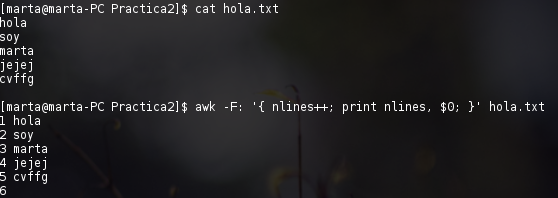
\includegraphics[width=0.7\textwidth]{2_49}
    \caption{Ejemplo de uso del comando \texttt{awk}}
    \label{awkej}
\end{figure}

\section{Práctica 3}
\subsection{Indique qué comandos ha utilizado para realizar la sustitución del disco RAID1 dañado por uno nuevo así como capturas de pantalla del proceso de reconstrucción del RAID.}
Para hacerlo vamos a seguir los pasos indicados en el guión de prácticas:
\begin{enumerate}[1.]
    \item En primer lugar, vamos a la configuración de la máquina virtual y añadimos un segundo disco. Nos tiene que quedar como se ve en la \hyperref[newdisk]{Figura \ref*{newdisk}}.

    \begin{figure}[!h]
    \centering
    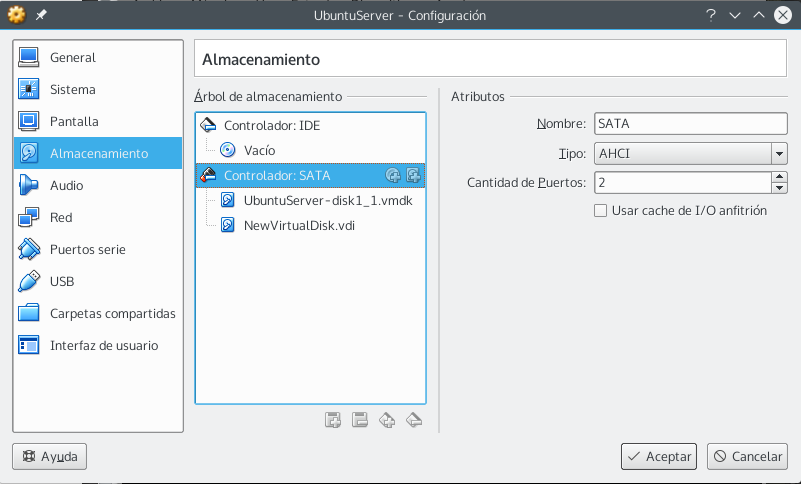
\includegraphics[width=0.7\textwidth]{3_3}
    \caption{Configuración de la máquina virtual tras añadir un nuevo disco}
    \label{newdisk}
    \end{figure}

    Tras añadir el disco, veremos el mensaje que se ve en la \hyperref[mensaje]{Figura \ref*{mensaje}}.
    \begin{figure}[!h]
        \centering
        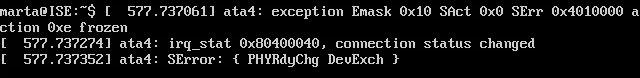
\includegraphics[width=0.7\textwidth]{3_4}
        \caption{Mensaje tras añadir un nuevo disco duro en caliente}
        \label{mensaje}
    \end{figure}

    \item Usamos el comando \texttt{mdadm} para eliminar el disco defectuoso del RAID y añadir el nuevo. Consultando \cite{mdadm}, vemos que para eliminar dispositivos del RAID podemos usar la opción \texttt{--remove} y para añadir, la opción \texttt{--add}.

    Primero, tenemos que consultar los discos que tenemos en nuestro ordenador, para ello usamos el comando \texttt{lsblk}. Obtenemos el output de la \hyperref[lsblk]{Figura \ref*{lsblk}}, en el cual vemos que el disco actual es el \texttt{sda1} y el que hemos insertado nuevo, \texttt{sdb}. También hemos consultado todos los dispositivos que tenemos en el sistema para saber cuál eliminar, en este caso sería \texttt{sda}.

    \begin{figure}[!h]
        \centering
        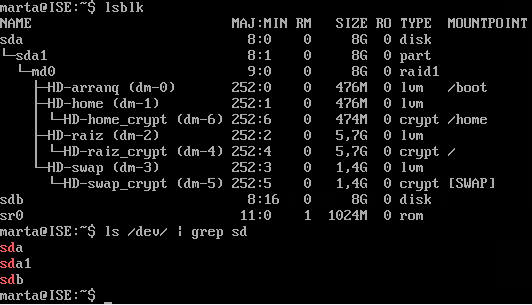
\includegraphics[width=0.7\textwidth]{3_5}
        \caption{Consultando cómo está el disco particionado y los discos que tenemos.}
        \label{lsblk}
    \end{figure}

    Con esa información, ejecutamos el comando \texttt{mdadm}:

\begin{minted}[frame=single, label={Eliminando el disco defectuoso y añadiendo el nuevo}]{bash}
sudo mdadm /dev/md0 --add /dev/sdb --remove /dev/sda    
\end{minted}

    Tras ejecutarlo, nos dice que se ha añadido con éxito el disco que hemos añadido nuevo, pero que no se ha encontrado el disco que íbamos a eliminar. Aún así, vemos que la ejecución ha sido exitosa en la \hyperref[finaloutput]{Figura \ref*{finaloutput}}.

    \begin{figure}[!h]
        \centering
        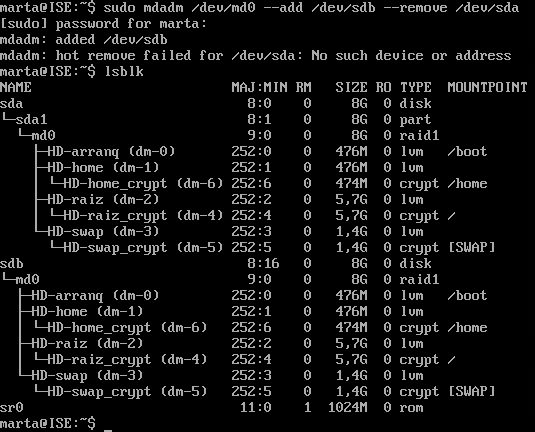
\includegraphics[width=0.7\textwidth]{3_6}
        \caption{Consultando cómo ha quedado particionado el disco tras añadir el disco nuevo al RAID}
        \label{finaloutput}
    \end{figure}
\end{enumerate}

\subsection{Instale \textit{Nagios} en su sistema (el que prefiera) documentando el proceso y muestre el resultado de la monitorización de su sistema comentando qué aparece.}
\subsubsection{Instalación}
En \cite{installnagios} se documenta paso a paso cómo instalar \textit{Nagios} en CentOS. Los pasos a seguir son los siguientes:
\begin{enumerate}[1.]
    \item En primer lugar, nos vamos al directorio temporal para trabajar desde ahí:
    \begin{minted}[frame=single, label={Accediendo al directorio /tmp}]{bash}
    cd /tmp
    \end{minted}

    \item Descargamos la última versión estable de \textit{Nagios}:
    \begin{minted}[frame=single, label={Descargando la última versión estable de Nagios}]{bash}
    wget http://assets.nagios.com/downloads/nagiosxi/xi-latest.tar.gz
    \end{minted}

    \item Extraemos el archivo que hemos descargado:
    \begin{minted}[frame=single, label={Extrayendo el contenido del archivo descargado}]{bash}
    tar xzf xi-latest.tar.gz
    \end{minted}

    \item Una vez extraído el archivo vamos al directorio de nagios:
    \begin{minted}[frame=single, label={Accediendo al directorio de nagios}]{bash}
    cd nagiosxi/
    \end{minted}

    \item Tras esto ejecutamos el script de instalación:
    \begin{minted}[frame=single, label={Ejecutando el script de instalación}]{bash}
    sudo ./fullinstall
    \end{minted}

    A mitad de instalación nos pedirá la contraseña para MySQL.

    \item Una vez instalado, para acceder a nagios basta con acceder a la dirección \texttt{localhost} o a la IP de nuestro servidor:
    \begin{minted}[frame=single, label={Accediendo a nagios desde Firefox}]{bash}
    firefox http://10.0.2.10/
    \end{minted}

    Una vez hecho eso, veremos la página de la \hyperref[paginicialnagios]{Figura \ref*{paginicialnagios}}.

    \begin{figure}[!h]
        \centering
        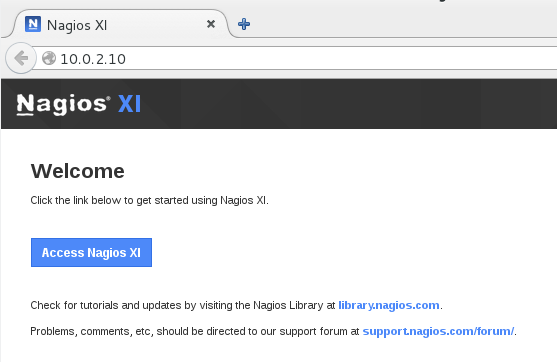
\includegraphics[width=0.5\textwidth]{3_29}
        \caption{Página inicial de Nagios}
        \label{paginicialnagios}
    \end{figure}

    \item Hacemos click en \textit{Access Nagios} y nos saldrá una ventana como la de la \hyperref[ventanainstall]{Figura \ref*{ventanainstall}} en la que debemos establecer algunos parámetros del sistema antes de empezar a usarlo.

    \begin{figure}[!h]
        \centering
        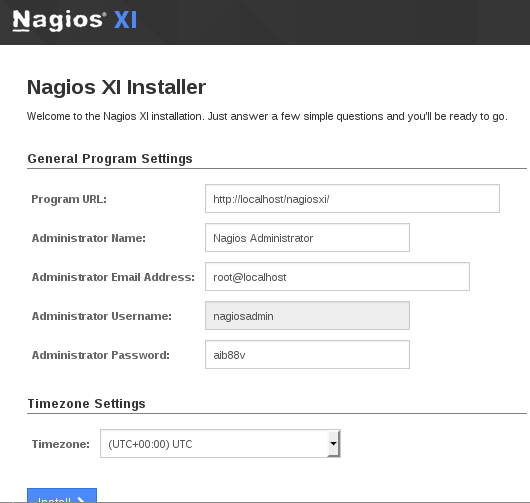
\includegraphics[width=0.5\textwidth]{3_30}
        \caption{Modificando algunos parámetros de Nagios antes de iniciar el sistema por primera vez}
        \label{ventanainstall}
    \end{figure}

    \item Por último nos mostrará una ventana con nuestro nombre de usuario y contraseña para acceder al sistema. Haciendo click en \textit{Login Nagios XI} e introduciendo el nombre de usuario y contraseña proporcionados, ya habremos terminado la instalación.

    \item Tras acceder al sistema deberemos de aceptar la licencia y tras aceptar la licencia nos dará un pequeño tutorial inicial. La interfaz inicial de \textit{Nagios} se ve en la \hyperref[interfaznagios]{Figura \ref*{interfaznagios}}.

    \begin{figure}[!h]
        \centering
        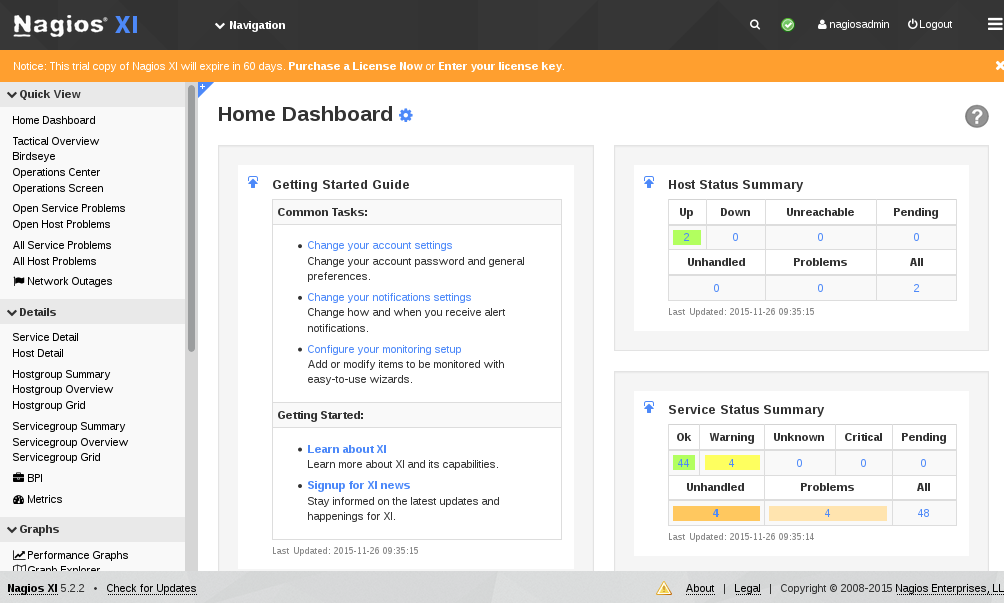
\includegraphics[width=0.5\textwidth]{3_31}
        \caption{Interfaz de Nagios al acceder al sistema}
        \label{interfaznagios}
    \end{figure}
\end{enumerate}

\subsubsection{Monitorización del sistema}
En el menú de la izquierda, tenemos algunas de las operaciones que podemos realizar con \textit{Nagios}. Por ejemplo, en el submení \textit{Service Detail}, podemos comprobar el estado de cada uno de los servicios que tenemos a activos en el sistema, incluyendo el propio \textit{Nagios} y el estado del propio sistema. En la \hyperref[monit]{Figura \ref*{monit}} se ve el ejemplo realizado por nosotros, en el que obtenemos varias advertencias sobre el poco espacio en disco que nos queda.

\begin{figure}[!h]
\centering
\mbox {
\subfigure[Resumen del estado de los servicios del sistema]{
\label{resumenservicios}
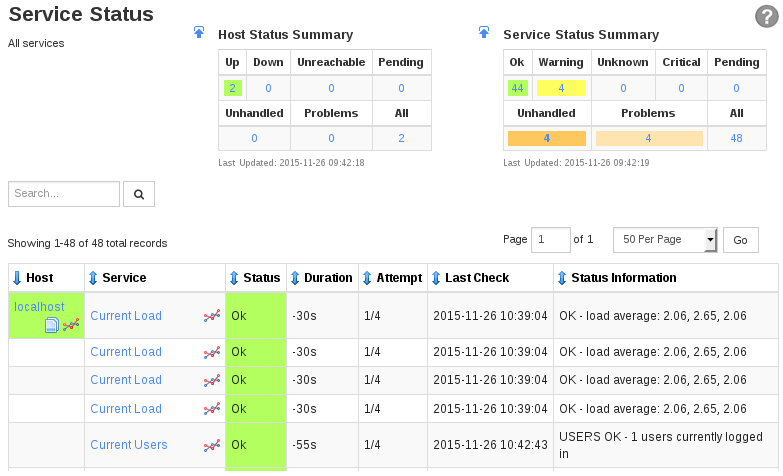
\includegraphics[width=0.5\textwidth]{3_33}
}
\qquad
\subfigure[Parte de la tabla detallada sobre cada servicio con varias advertencias] {
\label{advertenciasdisco}
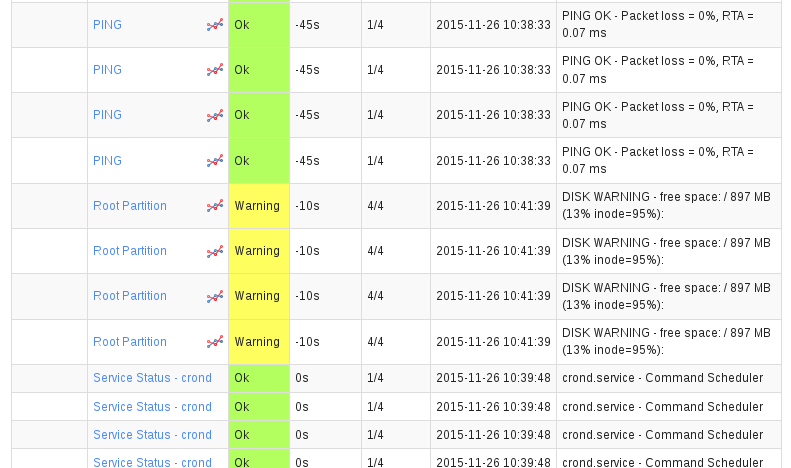
\includegraphics[width=0.5\textwidth]{3_32}
}
}
\caption{Monitorizando el estado de los servicios del sistema y del propio sistema}
\label{monit}
\end{figure}

En el submenú \textit{Metrics}, podemos obtener gráficas y datos sobre el uso de CPU, de memoria, de disco, de swap y la carga del sistema. En la \hyperref[swapuse]{Figura \ref*{swapuse}} estamos monitorizando el uso de la memoria de intercambio en el sistema, que en este caso vemos que tiene un uso aceptable y que no está saturada ya que tenemos un 54\% de memoria libre.

\begin{figure}[!h]
\centering
\mbox {
\subfigure[Resumen del uso de swap en el sistema]{
\label{swap}
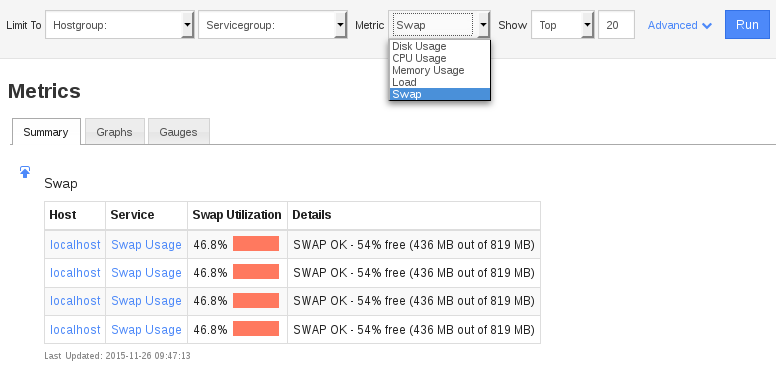
\includegraphics[width=0.5\textwidth]{3_34}
}
\qquad
\subfigure[Gráfica del uso de swap en el sistema] {
\label{semanapr}
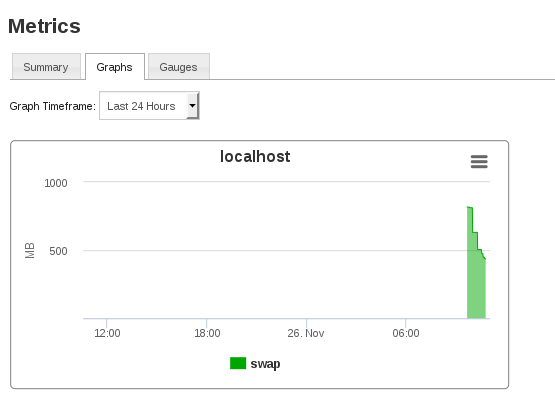
\includegraphics[width=0.5\textwidth]{3_35}
}
}
\caption{Monitorizando el uso de swap en el sistema}
\label{swapuse}
\end{figure}

\begin{figure}[!h]
\centering
\mbox {
\subfigure[Gráfico resumen de las veces que nuestro sistema no ha sido accesible]{
\label{salud}
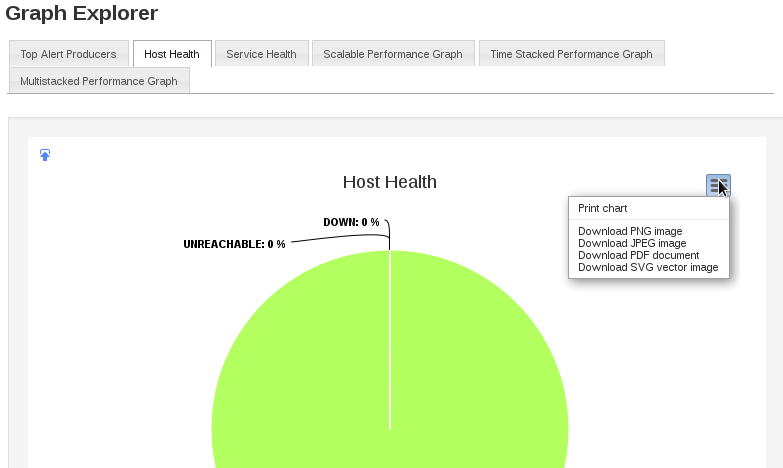
\includegraphics[width=0.5\textwidth]{3_37}
}
\qquad
\subfigure[Gráfico que hemos descargado en formato PNG sobre la ``salud'' de nuestro sistema] {
\label{graficopng}
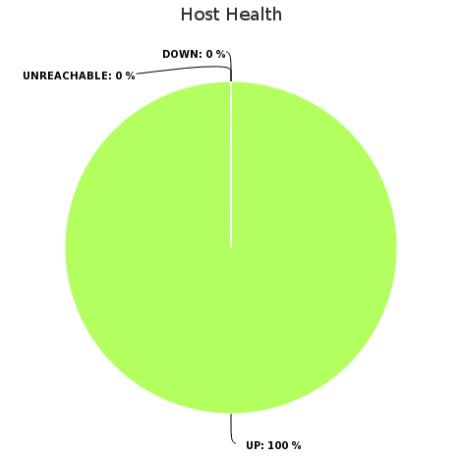
\includegraphics[width=0.3\textwidth]{3_38}
}
}
\caption{Monitorizando la ``salud'' del sistema}
\label{health}
\end{figure}

En el submenú \textit{Graph Explorer}, podemos consultar algunos gráficos realizados por \textit{Nagios} sobre nuestro servidor y nuestro sistema. En la \hyperref[salud]{Figura \ref*{salud}} se muestra un gráfico que muestra el número de veces que nuestro servidor ha estado innacesible (o bien porque se ha saturado, o porque se ha perdido la conexión, etc). En este caso, nuestro servidor ha estado siempre accesible y por eso muestra toda la gráfica en color verde. Además, \textit{Nagios} nos permite descargar el gráfico en varios formatos, por ejemplo en la \hyperref[graficopng]{Figura \ref*{graficopng}} se ve el archivo PNG de la gráfica descargado directamente desde \textit{Nagios}.

\subsection{Acceda a la demo online de \textit{Ganglia} de WikiMedia y haga lo mismo que hizo con \textit{Munin}}
En \href{http://ganglia.wikimedia.org/latest/}{WikiMedia} nos ofrecen una demo online del profiler \textit{Ganglia}, mostrándonos datos reales de sus servidores.

Nada más entrar a la página, nos encontramos con la página que se ve en la \hyperref[wikimediainfo]{Figura \ref*{wikimediainfo}} vemos un resumen estadístico del grid que usa WikiMedia, con el número total de CPUs y servidores tanto activos como no activos. También nos ofrecen una estadística sobre la carga desde los últimos 15 minutos y la utilización media. A la derecha de éstos datos vemos cuatro gráficas con datos sobre la carga del sistema, el uso de memoria, de CPU y de red. El uso de memoria sí es algo alto (más de la mitad), pero tanto la carga del sistema como el uso de CPU es bastante bajo. El uso de red tiene picos que varían bastante, por ejemplo, desde las 20:40 hasta las 21:00 no ha tenido actividad ninguna, sin embargo, sí ha tenido un pico de actividad a las 9.

\begin{figure}[!h]
    \centering
    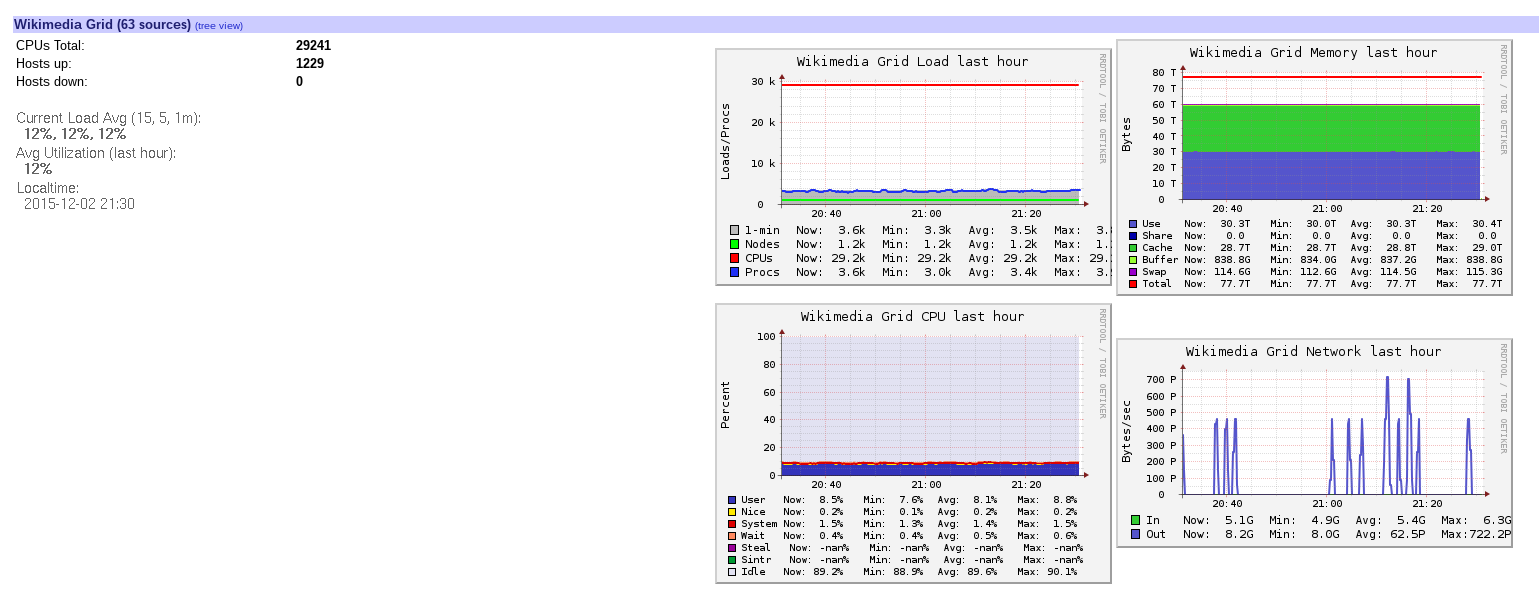
\includegraphics[width=1\textwidth]{3_50}
    \caption{Información general del grid de WikiMedia}
    \label{wikimediainfo}
\end{figure}

Después de esto, nos encontramos información sobre cada cluster de computadores de los que dispone WikiMedia (\textit{codfw} y \textit{equiad}). Si hacemos click en una de las gráficas, accedemos a una página en la que nos muestra información general sobre ese clúster, pero, dentro de dicha página podemos elegir ver información individual sobre un nodo concreto del clúster. Ésto se ve en la \hyperref[codfw]{Figura \ref*{codfw}}. Si elegimos un \textit{host}, vemos que tiene unas gráficas de rendimiento bastate parecidas a las del cluster (\hyperref[codfwhost]{Figura \ref*{codfwhost}}).

\begin{figure}[!h]
    \centering
    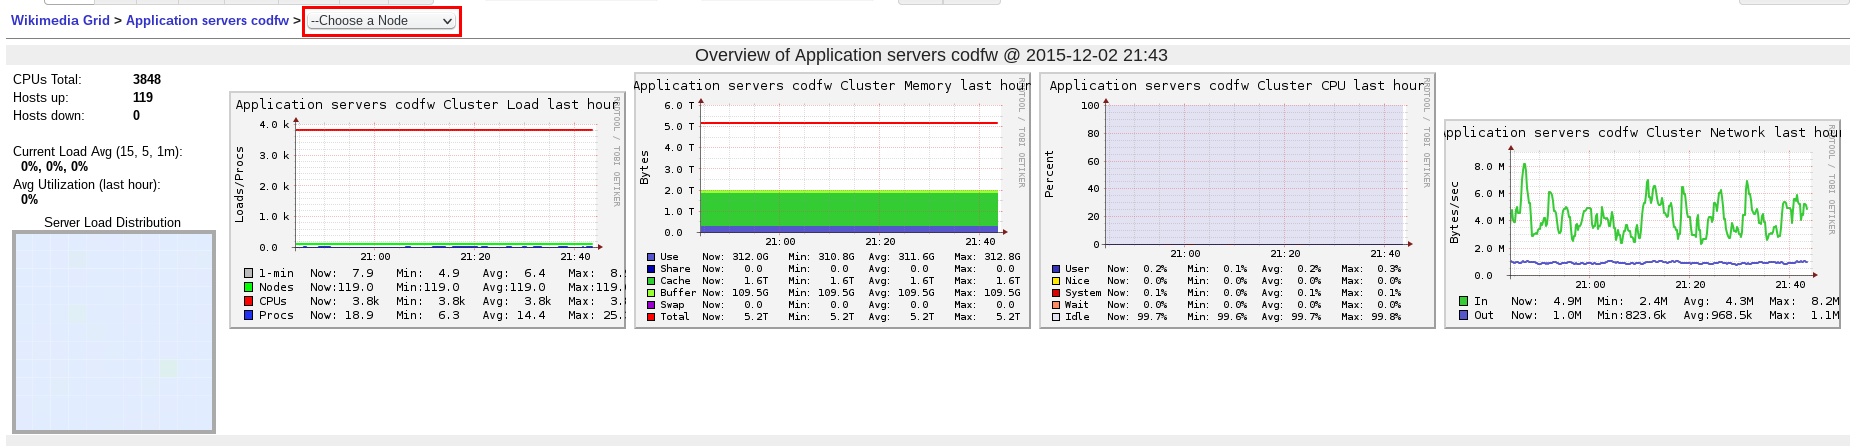
\includegraphics[width=1\textwidth]{3_51}
    \caption{Información general sobre los servidores de aplicación del clúster codfw}
    \label{codfw}
\end{figure}

\begin{figure}[!h]
    \centering
    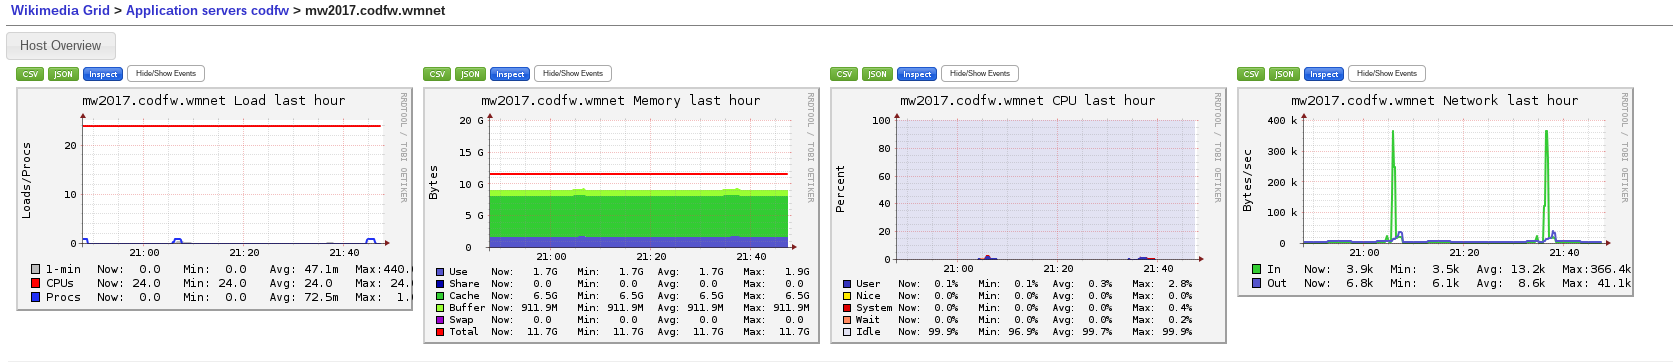
\includegraphics[width=1\textwidth]{3_52}
    \caption{Información general sobre uno de los hosts del clúster codfw}
    \label{codfwhost}
\end{figure}

\setcounter{subsection}{8}
\subsection{Escriba un script en python y analice su comportamiento usando el profiler presentado}
El script realizado consiste en cifrar usando el código de Polibio\cite{polibio}. El script en cuestión es el siguiente:

\newpage
\mypython[label={polibio.py}]{polibio.py}

Para hacer el profiling he usado la librería \textit{cProfile}, la cual, según \cite{pyprofile}, se usa con el siguiente comando:

\begin{minted}[frame=single,label={Haciendo profile a un script en Python}]{bash}
python -m cProfile polibio.py
\end{minted}

de forma análoga también podemos usar la librería \textit{profile}, con la cual obtenemos también la misma salida.

Tras ejecutar el comando anterior, he obtenido la salida que se ve en la \hyperref[outputprofile]{Figura \ref*{outputprofile}}. En primer lugar, el \textit{profiler} nos muestra el número de llamadas a funciones que ha realizado nuestro programa y el tiempo total de ejecución. El tiempo es tan alto debido a que también cuenta el tiempo que el programa ha estado dormido esperando la entrada desde teclado.

Por último, nos muestra cada una de las funciones a las que ha llamado nuestro programa junto al número de veces que se ha llamado a cada función. Por ejemplo, las dos funciones que incluye el script (\texttt{descrifrado\_colibio} y \texttt{cifra\_polibio}) se llaman una única vez cada una, como debe de ser pues en el script sólo se hace una llamada a cada función. También se reflejan llamadas a métodos primitivos de Python tales como \texttt{index}, \texttt{append}, etc los cuales se llaman más veces debido a que se llaman dentro de bucles \texttt{for}, en concreto, números relacionados con el tamaño de la frase a cifrar introducida.

\begin{figure}[!h]
    \centering
    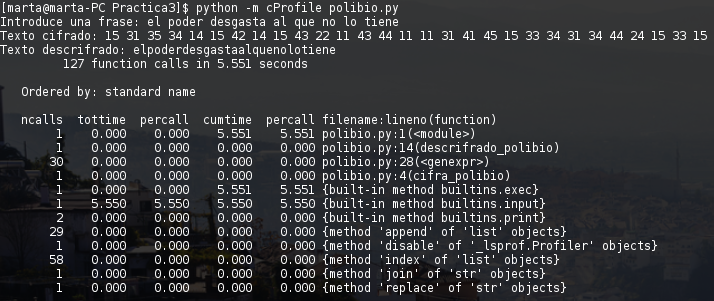
\includegraphics[width=1\textwidth]{3_42}
    \caption{Salida obtenida tras ejecutar \textit{cProfile} sobre un script Python}
    \label{outputprofile}
\end{figure}

\section{Práctica 4}
\subsection{Seleccione, instale y ejecute un benchmark, comente los resultados. \textbf{Atención}: no es lo mismo un benchmark que una suite, instale un benchmark}
En nuestro caso, de toda la lista de benchmarks disponibles, hemos elegido uno para medir la capacidad de la CPU para comprimir video usando la librería \texttt{x264} (\cite{x264}). Para instalarlo, según \cite{phoronixubuntu}, usamos el siguiente comando:
\begin{minted}[frame=single, label={Instalando el benchmark x264}]{bash}
sudo phoronix-test-suite benchmark x264
\end{minted}

tras esto, empezará a descargar e instalar el benchmark y sus dependencias. Una vez instalado nos mostrará el sofware y hardware de nuestra máquina y nos preguntará si queremos guardar la información en un fichero y si le decimos que no, empezará a hacer pruebas. En la prueba que hemos hecho en la \hyperref[x264test]{Figura \ref*{x264test}}, el benchmark nos da como conclusión que podríamos codificar unos 26 \textit{frames} por segundo. 

\begin{figure}[!h]
\centering
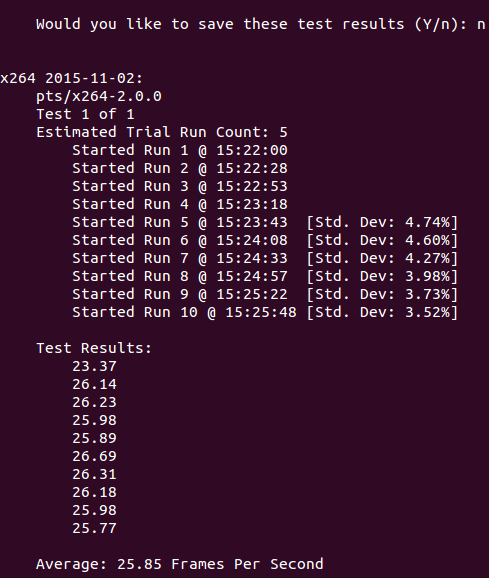
\includegraphics[width=0.5\textwidth]{4_3}
\caption{Salida del benchmark \texttt{x264} mientras realiza sus pruebas}
\label{x264test}
\end{figure}

\setcounter{subsection}{2}
\subsection{Lea el artículo de comparación entre \textit{Jmeter} y \textit{Gatling} elaborado por la empresa \textit{Flood.io} y elabore un breve resumen}
En \textit{Flood.io} no se fían de los benchmark ``competitivos'' ya que están hechos para favorecer a las empresas que lo patrocinan y no dan resultados realmente fiables. Por eso, se pasaron al lado del código abierto y probaron \textit{Jmeter} y \textit{Gatling}.

Tras hacer el \textit{test plan} con los dos benchmark, en el cual había 10.000 usuarios y 30.000 peticiones por minuto, el resultado obtenido es que ambos benchmark son bastante parecidos pero tienen una diferencia: \textit{Gatling} no es capaz de guardar el tamaño en bytes de la respuesta, pero sin embargo, a pesar de que \textit{Jmeter} sí lo es consume más recursos de CPU y memoria.

El artículo concluye diciendo que ambos benchmark son muy parecidos en términos de concurrencia y \textit{throughput} y que la elección de uno u otro es puramente subjetiva y hecha sobre alguna otra característica que cada herramienta incluya.

\bibliography{Opcionales} %archivo citas.bib que contiene las entradas 
\bibliographystyle{siam} % hay varias formas de citar

\end{document}